\chapter{Avaliação}
\label{cap:avaliacao}

Antes de se utilizar um novo sistema, é conveniente proceder-se a testes alargados de verificação e avaliação, com o objectivo de tomar conhecimento do seu correcto funcionamento e das sobrecargas introduzidas, para que possa ser utilizado como uma mais–valia.
O mecanismo implementado (\textit{MRoP}) foi avaliado funcionalmente, através de diversos testes aos dados de entrada, nos diversos componentes que o constituem.
Como existem diversas fontes de dados para o \textit{MRoP} (dados de controlo, dados do processo alvo de monitorização, fluxos de rede, etc.), foram criados vários testes de modo a que todas estas fontes de dados fossem analisadas.
Para além destas fontes directas de dados foi, igualmente, verificada a correcção de que todos os fluxos de dados obtidos, através da monitorização de rede, são exclusivos do processo alvo.
Assim todos estes testes e avaliações foram executados com sucesso e serão apresentados na secção \ref{sec:eval_functional}.

Como um dos principais objectivos desta dissertação é criar um mecanismo com melhor desempenho que os anteriores, apresentados na secção \ref{sect:outras_abordagens}, foi assim necessário verificar se este tinha sido atingido.
Para o efeito foram efectuados testes que serão apresentados na secção \ref{sec:eval_performance}, incidindo sobre o desempenho global na transferência de 1GB de dados, através de protocolos conhecidos, bem como através de outros testes que visam avaliar o mecanismo de instrumentação e a estrutura de dados escolhida para manter o estado do processo alvo.

Por último, serão apresentadas na secção \ref{sec:five_chap_conclusion} algumas conclusões sobre as análises efectuadas ao \textit{MRoP}.

\section{Avaliação Funcional}
\label{sec:eval_functional}

A análise funcional ao \textit{MRoP} teve várias vertentes, uma vez que este mecanismo recebe dados de diferentes fontes.
Assim os testes visaram a verificação dos dados inseridos pelo administrador, pelos dados monitorizados do processo alvo e os recolhidos das estruturas do núcleo.
Foi necessário garantir a inexistência de falhas nos mecanismo de entrada de dados no \textit{MRoP}, porque como este está a executar no núcleo tem acesso a todo o sistema, logo qualquer problema poderá comprometer o sistema quer ao nível de segurança quer ao nível de disponibilidade.
Foi igualmente verificado que, apesar da existência da instrumentação, a arquitectura de rede do núcleo \textit{Linux}, teve um comportamento correcto, produzindo os resultados esperados na sua avaliação.

\subsection{Teste ao componente de controlo}

Como o \textit{MRoP} foi desenvolvido para ser um módulo para o núcleo, foi necessário adicioná-lo a este, através do programa \textit{insmod}.
Após a inclusão do \textit{MRoP} ao núcleo, para que este funcione é necessário que um utilizador com permissões de administrador (\textit{root}), indique no ficheiro \textit{option}, criado no \textit{DebugFs} para o controlo do \textit{MRoP}, que deseja dar inicio à monitorização.
Dado que o \textit{MRoP} é parte do núcleo, é imprescindível garantir que a fiabilidade dos dados que lhe são transmitidos, não comprometem a segurança nem a disponibildade do sistema, pelo que as funções que recebem dados oriundos do sistema de controlo, efectuam verificações antes de os transmitirem às restantes componentes do \textit{MRoP}.
Como os dados de controlo são cadeias de caracteres, a função de verificação limita o comprimento máximo destes, baseado no valor máximo expectável para a utilização do ficheiro.
Assim cadeias de caracteres superiores a um determinado comprimento são truncadas, não existindo a possibilidade de explorar falhas de \textit{overflow}.
O valor zero (\textit{0}) serviu como inicializador, sendo que valores superiores a este, são indicadores de que existe uma opção activa no \textit{MRoP}.
Para além destas análises, foi também verificado que as permissões dos ficheiros são as estritamente necessárias e, restringem o seu acesso ao utilizador \textit{root}.

\subsection{Obtenção do estado dos canais do processo alvo}

A análise funcional de detecção dos protocolos, portos e endereços utilizados pelo(s) processo(s) alvo, foi efectuada recorrendo à criação de dois conjuntos de programas \textit{cliente/servidor}.
Para o primeiro conjunto foi criado um servidor e um cliente, ambos utilizando o protocolo \textit{tcp}, em que o programa servidor esperava conexões numa porta e endereço pré-definidos.
Como o \textit{MRoP} instrumenta as chamadas ao sistema \textit{connect}, \textit{accept}, \textit{bind}, \textit{recvfrom}, \textit{sendto} e a função \textit{sock\_close}, é possível capturar todas as operações relativamente às comunicações de rede utilizando os protocolos \textit{tcp} e \textit{udp}.
Nas chamadas ao sistema \textit{bind} e \textit{connect}, um dos seus argumentos é uma estrutura \textit{sockaddr} que contém informações sobre o endereço e porto, sendo que na função \textit{connect} estes são relativos ao destino, e na função \textit{bind} são relativos à origem.
Assim os dados anteriormente mencionados, são utilizados na construção do repositório do \textit{MRoP}, de modo a capturar apenas o tráfego respeitante ao processo alvo.
Como os dados são provenientes do processo alvo, não é possível garantir a sua fiabilidade, assim caso a função instrumentada retorne com um valor de erro, os dados anteriormente adicionados (porto, endereço e protocolo) são retirados do repositório, ficando novamente num estado consistente com o processo alvo.
De modo a verificar que os dados que se encontram no repositório estão correctos, estes podem ser apresentados através da função \textit{printk} para o terminal do núcleo, ou podem ser apresentados no ficheiro criado para o efeito no sistema de ficheiros virtual \textit{DebugFs}, podendo confirmar a sua exactidão com o que a aplicação \textit{netstat} apresenta para a aplicação alvo, ou confrontado com o esperado, tendo em conta o seu código fonte.

Quando o processo alvo já se encontra em execução e se inicia a monitorização, os \textit{sockets} que já estejam em utilização contêm os dados relativos aos protocolos, portos e endereços dos \textit{sockets} e, por isso consideram-se correctos e válidos, sendo automaticamente adicionados ao repositório.
As verificações efectuadas para as várias situações permitiram confirmar o correcto funcionamento do sistema.

\subsection{Avaliação de monitorização de rede}

Foi efectuada uma verificação à correcção dos dados transferidos entre dois processos, um cliente, outro servidor e respectivos pacotes capturados pelo sistema.
Estes testes foram apenas efectuados para protocolos assentes sobre \textit{tcp}, pois nestes existe a certeza que, devido ao sistema de controlo de comunicação não existem falhas, o que permite analisar a transferência do início ao fim e comparar com os dados originais dos ficheiros transferidos.

A execução do teste consistiu na transferência de um ficheiro entre duas máquinas, ligadas por um \textit{switch} com portas a 100 \textit{Mbit/s}, através do protocolo aplicacional \textit{ftp}, enquanto existiam outros fluxos de rede de outros processos.
Foi escolhido este protocolo pois, apesar de ser necessário conhecer \textit{à priori} a porta de comunicação com o servidor, a transmissão de dados é efectuada noutra porta negociada dinamicamente, permitindo demonstrar também o potêncial do \textit{MRoP}.
Todas as comunicações remotas referentes a esta transferência foram monitorizadas através do programa \textit{tcpdump}, com o módulo do núcleo \textit{MRoP} activo e com a indicação do processo a monitorizar.
Esta monitorização foi guardada através do \textit{tcpdump} num ficheiro para posterior análise através do \textit{Wireshark}.
Utilizando o ficheiro capturado no \textit{Wireshark}, foi possível observar que apenas os fluxos de rede da transferência foram capturados.
Após esta verificação, foi efectuada a recuperação do ficheiro transmitido através da agregação dos dados presentes nos pacotes capturados, exceptuando os cabeçalhos.
Esta recuperação foi guardada num ficheiro temporário, de modo a poderem ser aplicadas funções de síntese (\textit{md5} e \textit{sha1}), com o objectivo de verificar se o conteúdo dos pacotes recuperado era exactamente igual ao do ficheiro original, e à sua transferência.
Esta verificação foi confirmada através do retorno do mesmo valor para os três ficheiros, para cada uma das funções de síntese utilizadas.

Foi igualmente verificada a correcção das transferências sobre o protocolo \textit{udp}, para o que se procedeu à realização de um teste utilizando o programa \textit{iperf}, com recurso a \textit{sockets} \textit{udp}.
Para a realização do referido teste recorreu-se à mesma infra-estrutura de rede, em que numa das máquinas foi executado o \textit{iperf} em modo servidor utilizando \textit{sockets udp}, enquanto na outra foi executado o modo cliente utilizando \textit{sockets} \textit{udp}.
Foi ainda efectuada a monitorização de rede na máquina que executou o \textit{iperf} em modo cliente, através do programa \textit{tcpdump} com o módulo do núcleo activo e com a indicação do identificador do processo \textit{iperf}, enquanto existiam outros fluxos de rede de outros processos.
O resultado da monitorização pelo \textit{tcpdump} foi guardado num ficheiro, que indicou que o total de \textit{bytes} correctamente recebidos pelo \textit{iperf} em modo servidor, foram igualmente obtidos pela monitorização.
Neste ficheiro também não existiam outros fluxos de dados que não os respeitantes à utilização do \textit{iperf}.

Como anteriormente referido, aquando da realização dos testes existiram outros fluxos de rede, nomeadamente de tráfego \textit{web}, e de aplicações de conversação instantânea, entre outros, de modo a comprovar a eficácia do \textit{MRoP}.

\section{Avaliação do desempenho}
\label{sec:eval_performance}

Tendo em vista a avaliação do desempenho, foram efectuados diversos testes com o objectivo de avaliar a sobrecarga gerada pela introdução do \textit{MRoP}.
Estes testes basearam-se na recepção ou transmissão de \textit{1 GigaByte} de dados, utilizando diferentes programas e protocolos, entre duas máquinas ligadas directamente.
Ambas as máquinas, que se optou por designar de máquina 1 e máquina 2, procederam à transmissão/recepção de dados, utilizando cada uma, apenas, um processador activo de 2 e de 2.6 Ghz, respectivamente, por forma a evitar que a sobrecarga introduzida fosse repartida pelos dois cores, mascarando assim a eventual perda de desempenho.
As máquinas anteriormente referidas encontravam-se conectadas directamente, por interfaces de rede a 100 MBit/s, ficando uma responsável pela execução dos servidores \textit{ftp}, \textit{http} e \textit{iperf}, e a outra pelos respectivos clientes.
A versão do sistema de operação utilizado, em ambas as máquinas, correspondeu ao 2.6.39, sendo que na máquina 1 foram introduzidas as modificações, para incluir o \textit{MRoP} e as suas funções auxiliares, enquanto na máquina 2 se executou o sistema original.

\subsection{Desempenho do \textit{MRoP}}

Na execução destes testes, foram efectuadas dez iterações, isto é, cada teste foi executado dez vezes, para cada experiência considerada, de modo a obter um valor médio e um desvio padrão considerado aceitável.
Os testes efectuados, em particular os primeiros, não mostraram desvantagem em ter o mecanismo \textit{MRoP} activo, com vista a medir a sobrecarga do \textit{MRoP}.
Os resultados obtidos constam nas tabelas \ref{tab:desempenho} e \ref{tab:overhead}.

Os primeiros quatro testes foram efectuados utilizando apenas uma conexão ao servidor, enquanto o 5º e o 6º testes utilizaram mais uma comunicação, de modo a aumentar o peso sobre o processador, sobre os sistemas de operação e o número de pacotes a circular entre as máquinas.
Desta forma, foi possível identificar a sobrecarga exercida enquanto o \textit{tcpdump} executava e capturava todos os pacotes (sistema original) ou apenas um subconjunto destes, no novo sistema, os pacotes relativos aos processos alvo.

Na tabela \ref{tab:desempenho}, a coluna "Original" corresponde aos valores resultantes dos tempos médios das execuções das transferências na ausência de monitorização.
Na mesma tabela e na coluna "Com \textit{TcpDump}", é apresenta a média dos tempos de transferência com a captura total do tráfego utilizando a biblioteca \textit{PCap}/\textit{LSF} original, enquanto que a coluna identificada com "Com \textit{TcpDump} e \textit{MRoP}" regista a média dos tempos para a transferência com captura pelo tcpdump e o módulo \textit{MRoP} desenvolvido no núcleo, de forma a capturar, apenas, o tráfego da transferência do processo alvo.
Nos primeiros quatro testes é possível verificar que a utilização do \textit{MRoP}, aumentou de forma irrelevante o tempo de execução (figura \ref{fig:tests_graphics}).

\begin{figure}[!htbp]
\centering
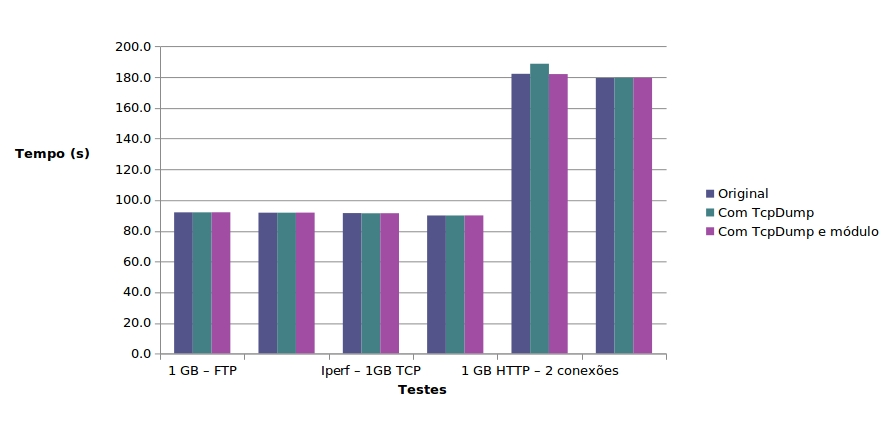
\includegraphics[scale=0.6]{testes.jpg}
\caption{Testes de desempenho efectuados ao MRoP}
\label{fig:tests_graphics}
\end{figure}

É igualmente possível observar que no 1º e 3º testes, aquando da utilização do \textit{tcpdump}, a execução sem o \textit{MRoP}, mostrou-se ligeiramente mais rápida, como se pode verificar na tabela \ref{tab:desempenho} e \ref{tab:overhead}.
\begin{table}[!htb]
\begin{center}
\caption{Tempos médios em segundos (s)}
\begin{tabular}{ | c | c | c | c |  }
\hline
Teste & \hspace {0.3cm} Original \hspace {0.3cm}& \hspace {0.2cm} Com TcpDump \hspace {0.2cm} & Com TcpDump e MRoP \\
\hline
1GB - FTP$^{1}$ & 91.8508	& 91.8500 & 91.8854 \\
1GB - HTTP$^{2}$ & 91.6391 & 91.6472 & 91.6674 \\ 
IPerf - 1GB TCP$^{3}$ & 91.3790	& 91.2535	& 91.2672 \\
IPerf - 1GB UDP$^{4}$ & 89.7975 & 89.8007 & 89.8464 \\
\hline
\hline
1GB HTTP - 2 conexões$^{5}$ & 182.1573 & 188.7156 & 182.0161 \\
IPerf - 1GB UDP 2 conexões$^{6}$ & 179.4930 & 179.6280 & 179.6369 \\
\hline
\end{tabular}
\label{tab:desempenho}
\end{center}
\end{table}
Esta situação deve-se ao facto de, quando a máquina se encontra em sobrecarga, leva ao aumento do tamanho médio dos pacotes, reduzindo o seu número e o volume de dados transferidos, em virtude da diminuição dos seus cabeçalhos.
Este comportamento já tinha sido detectado numa dissertação anterior~\cite{Farruca:2009}.

Nos 5º e 6º testes, como o tráfego na interface é duplicado e o \textit{tcpdump} tem que capturar todos os pacotes, é possível evidenciar a sobrecarga exercida por estas cópias de dados e consequentes transferências (para nível utilizador) face ao novo sistema onde apenas captura um fluxo de dados.

Na tabela \ref{tab:overhead} e na figura \ref{fig:tests_overhead} é possível observar que, para o teste 5, a sobrecarga do \textit{tcpdump} atinge os 3.6\% face ao original, enquanto que a sobrecarga do \textit{tcpdump} com o \textit{MRoP}, permitiu uma ligeira melhoria face ao original (-0.0775\%).
Conclui-se, portanto, que quando o fluxo de dados que não pretendemos capturar aumenta consideravelmente, torna-se mais vantajoso utilizar o \textit{MRoP}, do que capturar todos os pacotes.
Este modo de captura minimiza a sobrecarga, capturando apenas os dados relevantes, evitando-se a identificação e filtragem dos pacotes pertencentes ao processo alvo em nível utilizador, tendo como consequência uma sobrecarga adicional.

\begin{figure}[!ht]
\centering
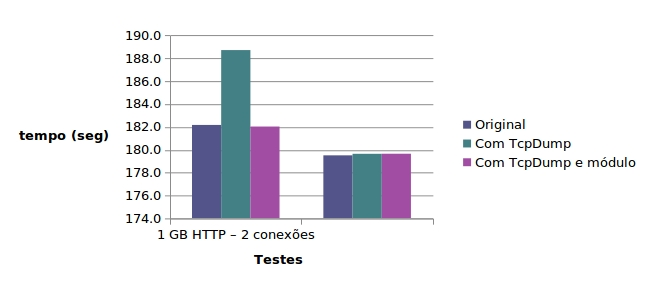
\includegraphics[scale=0.7]{overhead.jpg}
\caption{Sobrecarga nos testes 5 e 6 }
\label{fig:tests_overhead}
\end{figure}


\begin{table}[!htb]
\begin{center}
\caption{Sobrecarga das transferências (valores em percentagem)}
\begin{tabular}{ | c | c | c |}
\hline
Teste & \hspace {0.3cm} TcpDump \hspace {0.3cm} & TcpDump com MRoP  \\

\hline
1GB - FTP$^{1}$ & -0.0009  & 0.0377  \\
1GB - HTTP$^{2}$ & 0.0088 &  0.0309   \\
IPerf - 1GB TCP$^{3}$ & -0.1373 &  -0.1223   \\
IPerf - 1GB UDP$^{4}$ & 0.0036 & 0.0545 \\
\hline
\hline
1GB HTTP - 2 conexões$^{5}$ & 3.6003 & -0.0775   \\
IPerf - 1GB UDP 2 conexões$^{6}$ & 0.0752 & 0.0802   \\
\hline
\end{tabular}
\label{tab:overhead}
\end{center}
\end{table}

Os resultados da sobrecarga do \textit{tcpdump} com o \textit{MRoP}, em todos os casos analisados, foram sempre inferiores a 0.15\%, chegando mesmo a atingir 0.0309\%.
Se compararmos este resultado com os obtidos em \cite{Farruca:2009}, assiste-se a uma substâncial melhoria.
Efectuando a comparação deste resultado com o obtido no 2º teste, da transferência por \textit{HTTP}, não por ser o melhor resultado obtido, mas por o teste ser idêntico, estamos perante uma melhoria no desempenho de 64 vezes.

Como o anteriormente referido, os testes realizados apenas com o \textit{tcpdump} capturam todo o tráfego e, como não existia a monitorização do processo alvo, não era efectuada a filtragem dos pacotes.
Desta forma os valores apresentados para o \textit{tcpdump} são meramente indicativos relativamente ao \textit{tcpdump} com o \textit{MRoP} activo, uma vez que lhe falta a componente de filtragem dos dados, aumentando o tempo de execução e a sua sobrecarga.

\subsection{Desempenho da estrutura de dados}

Para além das avaliações anteriormente descritas, procurou analisar-se o comportamento da estrutura de dados utilizada no componente \textit{Estado do processo}, de modo a verificar o seu desempenho.
Assim para esta análise, foi elaborado um teste para determinar o desempenho da estrutura de dados, relativamente às inserções e remoções.
Este teste utilizou o sistema de alta resolução de temporizadores (\textit{HRTimer})\cite{hrtimerKernel}, presente no núcleo do sistema de operação.

Para decidir qual o número de elementos a ser utilizado para este teste, foi verificado qual o valor máximo de descritores de canais que um processo pode ter.
O valor foi obtido através da função \textit{getrlimits}, que indicou que o valor máximo de descritores de canais abertos, para um processo, é de 1024 canais\footnote{é certo que este valor pode ser alterado na configuração do sistema de operação, mas considerou-se este um limite típico para a maioria das aplicações.}.
Dado que este valor (1024) é o máximo de canais por processo, considerou-se um óptimo valor para verificar o comportamento da estrutura de dados no pior caso, no cenário em que todos os descritores de canais são \textit{sockets} e estão activos.
Os valores obtidos através deste teste demonstraram os valores máximos espectáveis, em que se assume que o processo alvo está a utilizar o número máximo de canais de rede.

Assim o teste consistiu em obter o tempo anterior e posterior à inserção dos 1024 elementos, representando outros tantos portos/endereços, afim de determinar o tempo decorrido.
De igual modo, foi calculado o tempo de remoção dos referidos elementos.
Os resultados obtidos estão reproduzidos na tabela \ref{tab:tree_info}.
 
\begin{table}[!htb]
\begin{center}
\caption{Custo das operações (tempos em nanosegundos)}
\begin{tabular}{ | r | c | c | }
\hline
\hspace{1cm} Teste \hspace{1.5cm} & \hspace{1cm}Duração\hspace{1cm} &  Média por
elemento \\
\hline
Adição de 1024 elementos & 869 244 & 848.8711 \\
\hline
Remoção de 1024 elementos & 675 086 & 659.2637\\
\hline

\hline
\end{tabular}
\label{tab:tree_info}
\end{center}
\end{table}

Pode verificar-se, pela tabela \ref{tab:tree_info}, que a inserção de um elemento na árvore é inferior a 1 microsegundo, demonstrando que a estrutura utilizada não introduz uma elevada sobrecarga.
A inserção de dados no repositório, não é efectuada com um desempenho constante, dado que quando é necessário efectuar um rebalanceamento da árvore, o processo de inserção é mais demorado devido à necessidade de efectuar rotações na árvore.
Para além de estabelecer um bom compromisso de desempenho e utilização de memória, a sua disponibilidade de utilização no núcleo do sistema, possibilitou um elevado grau de confiança na sua utilização.

O tempo médio despendido na procura do elemento com o menor valor de chave, nos 1024 elementos adicionados, foi de 1327 nanosegundos.
Com este valor é possível verificar que para efectuar 10 iterações de procura na árvore, incorre-se numa penalização de 1.3 microsegundos.
Verifica-se que o tempo médio de procura de elementos na estrutura, é sempre menor ou igual a 1.3 microsegundos.
Considerando que a maioria das aplicações não utiliza tantos portos em simultâneo, são expectáveis tempos inferiores em aplicações reais.

O teste de desempenho realizado demonstra que, mesmo nas piores condições, ou seja nas condições mais extremas, consegue-se obter um desempenho aceitável.

\subsection{Desempenho do Sistema de instrumentação}
Sendo a instrumentação das chamadas ao sistema um dos pontos fundamentais na execução do \textit{MRoP}, a análise ao seu comportamento é deveras importante, na medida em que é necessário verificar se a introdução deste tipo de instrumentação irá produzir uma elevada penalização sobre o sistema de operação.
A titulo exemplificativo da sobrecarga introduzida pelo \textit{KRetProbe} em cada função instrumentada, foi adicionado \textit{KRetProbe} à chamada ao sistema \textit{getpid}.
Esta chamada ao sistema foi escolhida, devido à simplicidade da função que apenas devolve o identificador do processo que a invocou.
Este teste consistiu em avaliar o tempo decorrido entre o início e o fim do total das chamadas, com e sem o \textit{KRetProbe}, de forma a avaliar a sobrecarga e verificar a sua coincidência com o indicado pelos criadores do sistema.

\providecommand{\e}[1]{\ensuremath{\times 10^{#1}}}

\begin{table}[!htb]
\begin{center}
\caption{Duração das chamadas em segundos}
\begin{tabular}{ | c | c | c | c |}
\hline
Teste & Original & Com \textit{KRetProbe} & Sobrecarga por chamada\\
\hline
100 000 000 chamadas & 12.65 &  73.6600 & 610.10\e{-9}\\
1 000 000 000 chamadas & 126.85 & 737.2100 & 610.36\e{-9}\\
\hline
\end{tabular}
\label{tab:kprobes_info}
\end{center}
\end{table}

O valor de referência obtido pelos criadores do \textit{KProbes}, referentes ao \textit{KRetProbe} sem optimizações, é de 0.7 microsegundos\cite{KProbeKernel}, sendo que o valor médio obtido foi de 0.61 microsegundos, ou seja, ligeiramente inferior, visto que a máquina de referência apresenta uma frequência de \textit{cpu} inferior à máquina onde foram realizados estes testes.
Esta sobrecarga é constante para cada chamada ao sistema, sendo que qualquer melhoria ao \textit{KProbes} irá afectar positivamente a sobrecarga do \textit{MRoP}.

Consideram-se estes valores bastante aceitáveis e espera-se que tenham ainda reduzido impacto no desempenho normal do sistema.
Note-se ainda que a instrumentação só é introduzida aquando do carregamento do \textit{MRoP}, de modo a executar a monitorização com esta nova funcionalidade, não tendo por isso, o processo inicial de introdução da instrumentação, qualquer impacto durante o funcionamento do sistema.

\section{Conclusão}
\label{sec:five_chap_conclusion}

Com os testes efectuados ao nível funcional e ao nível de desempenho ao \textit{MRoP} verificou-se que este mecanismo oferece um desempenho aceitável nas condições mais adversas, o que indicia que para as condições das aplicações reais o seu desempenho será superior, enquanto que a sobrecarga introduzida no sistema poderá ser inferior ao constatado.

Pode verificar-se em relação ao trabalho \cite{Farruca:2009}, que a sobrecarga gerada pelo \textit{MRoP} foi muito inferior, demonstrando que apesar da dificuldade de operar no núcleo, criar um sistema de monitorização de rede orientado ao processo através de um mecanismo não intrusivo, que logo que possível rejeite a captura de pacotes irrelevantes, reduz consideravelmente a sobrecarga no sistema, mesmo relativamente ao \textit{LSF} / \textit{PCap} original.

Existe ainda a possibilidade de reduzir a sobrecarga no sistema, se ao invés de se instrumentar as chamadas ao sistema, forem instrumentadas as funções específicas relacionadas com a pilha de protocolos \textit{tcp/ip}.
